\bta{其它电学实验}


\begin{enumerate}
%\renewcommand{\labelenumi}{\arabic{enumi}.}
% A(\Alph) a(\alph) I(\Roman) i(\roman) 1(\arabic)
%设定全局标号series=example	%引用全局变量resume=example
%[topsep=-0.3em,parsep=-0.3em,itemsep=-0.3em,partopsep=-0.3em]
%可使用leftmargin调整列表环境左边的空白长度 [leftmargin=0em]
\item
\exwhere{$ 2019 $ 年物理全国\lmd{2}卷}
某小组利用图($ a $)所示的电路,研究硅二极管在恒定电流条件下的正向
电压 $ U $ 与温度 $ t $ 的关系,图中 $ V_{1} $ 和 $ V_{2} $ 为理想电压表;$ R $ 为滑动变阻器,$ R_{0} $ 为定值电阻(阻值 $ 100 \ \Omega $);
$ S $ 为开关,$ E $ 为电源。实验中二极管置于控温炉内,控温炉内的温度 $ t $ 由温度计(图中未画出)测
出。图($ b $)是该小组在恒定电流为 $ 50.0 \ \mu A $ 时得到的某硅二极管 $ U-I $ 关系曲线。回答下列问题:
\begin{figure}[h!]
\centering
\begin{subfigure}{0.4\linewidth}
\centering
\includesvg[width=0.7\linewidth]{picture/svg/GZ-3-tiyou-1039} 
\caption{}\label{}
\end{subfigure}
\begin{subfigure}{0.4\linewidth}
\centering
\includesvg[width=0.7\linewidth]{picture/svg/GZ-3-tiyou-1040} 
\caption{}\label{}
\end{subfigure}
\end{figure}

\begin{enumerate}
%\renewcommand{\labelenumi}{\arabic{enumi}.}
% A(\Alph) a(\alph) I(\Roman) i(\roman) 1(\arabic)
%设定全局标号series=example	%引用全局变量resume=example
%[topsep=-0.3em,parsep=-0.3em,itemsep=-0.3em,partopsep=-0.3em]
%可使用leftmargin调整列表环境左边的空白长度 [leftmargin=0em]
\item
实验中,为保证流过二极管的电流为 $ 50.0 \ \mu A $,应调节滑动变阻器 $ R $,使电压表 $ V_{1} $ 的示数为
$ U_{1} =$ \underlinegap $mV $;根据图($ b $)可知,当控温炉内的温度 $ t $ 升高时,硅二极管正向电阻 \underlinegap (填“变
大”或“变小”),电压表 $ V_{1} $ 示数 \underlinegap (填“增大”或“减小”)
,此时应将 $ R $ 的滑片向 \underlinegap (填“$ A $”或“$ B $”)
端移动,以使 $ V_{1} $ 示数仍为 $ U_{1} $。

\item 
由图($ b $)可以看出 $ U $ 与 $ t $ 成线性关系,硅二极管可以作为测温传感器,该硅二极管的测温灵
敏度为 $\left|\frac{\Delta U}{\Delta t}\right|=$ \underlinegap $ \times 10^{-3} \ V / \celsius $(保留 $ 2 $ 位有效数字)。




\end{enumerate}


\tk{
\begin{enumerate}
%\renewcommand{\labelenumi}{\arabic{enumi}.}
% A(\Alph) a(\alph) I(\Roman) i(\roman) 1(\arabic)
%设定全局标号series=example	%引用全局变量resume=example
%[topsep=-0.3em,parsep=-0.3em,itemsep=-0.3em,partopsep=-0.3em]
%可使用leftmargin调整列表环境左边的空白长度 [leftmargin=0em]
\item
$ 5.00 $ \quad 变小 \quad 增大 \quad $ B $
\item 
$ 2.8 $
\end{enumerate}
} 


\item 
\exwhere{$ 2015 $ 年上海卷}
在“用 $ DIS $ 研究通电螺线管的磁感应强度”实验中:
\begin{enumerate}
%\renewcommand{\labelenumi}{\arabic{enumi}.}
% A(\Alph) a(\alph) I(\Roman) i(\roman) 1(\arabic)
%设定全局标号series=example	%引用全局变量resume=example
%[topsep=-0.3em,parsep=-0.3em,itemsep=-0.3em,partopsep=-0.3em]
%可使用leftmargin调整列表环境左边的空白长度 [leftmargin=0em]
\item
在对螺线管通电 \underlinegap (选填“前”或“后”)必须对磁传感器进行调零。
\item 
(单选题)实验时,将磁传感器探管前端插至通电螺线管轴线中点时,磁传感器读数为 $ 5 \ m T $。
减小通电螺线管的电流后,将探管从螺线管的另一端插入,当探管前端再次到达螺线管轴线中点时,
磁传感器的读数可能为 \underlinegap .
\fourchoices
{$ 5 \ m T $}
{$ -5 \ m T $}
{$ 3 \ m T $}
{$ -3 \ m T $}



\end{enumerate}

\tk{
\begin{enumerate}
%\renewcommand{\labelenumi}{\arabic{enumi}.}
% A(\Alph) a(\alph) I(\Roman) i(\roman) 1(\arabic)
%设定全局标号series=example	%引用全局变量resume=example
%[topsep=-0.3em,parsep=-0.3em,itemsep=-0.3em,partopsep=-0.3em]
%可使用leftmargin调整列表环境左边的空白长度 [leftmargin=0em]
\item
前
\item 
D
\end{enumerate}
} 



\item 
\exwhere{$ 2015 $ 年理综山东卷}
如图甲所示的电路中,恒流源可为电路提供恒定电流 $ I_{0} $,$ R $ 为定值
电阻,电流表、电压表均可视为理想电表。某同学利用该电路研究滑动变阻器 $ R_{L} $ 消耗的电功率。
改变 $ R_{L} $ 的阻值,记录多组电流、电压的数值,得到如图乙所示的 $ U- I $ 关系图线。
回答下列问题:
\begin{figure}[h!]
\centering
\begin{subfigure}{0.4\linewidth}
\centering
\includesvg[width=0.7\linewidth]{picture/svg/GZ-3-tiyou-1041} 
\caption{}\label{}
\end{subfigure}
\begin{subfigure}{0.4\linewidth}
\centering
\includesvg[width=0.7\linewidth]{picture/svg/GZ-3-tiyou-1042} 
\caption{}\label{}
\end{subfigure}
\end{figure}



\begin{enumerate}
%\renewcommand{\labelenumi}{\arabic{enumi}.}
% A(\Alph) a(\alph) I(\Roman) i(\roman) 1(\arabic)
%设定全局标号series=example	%引用全局变量resume=example
%[topsep=-0.3em,parsep=-0.3em,itemsep=-0.3em,partopsep=-0.3em]
%可使用leftmargin调整列表环境左边的空白长度 [leftmargin=0em]
\item
滑动触头向下移动时,电
压表示数
\underlinegap 
(填“增大”或
“减小”)
。


\item 
$ I_{0} = $ \underlinegap $ A $。

\item 
$ R_{L} $ 消耗的最大功率
为
\underlinegap 
$ W $(保留一位有效数字)。




\end{enumerate}

\tk{
\begin{enumerate}
%\renewcommand{\labelenumi}{\arabic{enumi}.}
% A(\Alph) a(\alph) I(\Roman) i(\roman) 1(\arabic)
%设定全局标号series=example	%引用全局变量resume=example
%[topsep=-0.3em,parsep=-0.3em,itemsep=-0.3em,partopsep=-0.3em]
%可使用leftmargin调整列表环境左边的空白长度 [leftmargin=0em]
\item
减小
\item 
$ 1 $
\item 
$ 5 $
\end{enumerate}
} 


\item 
\exwhere{$ 2013 $ 年四川卷}
在探究两电荷间相互作用力的大小与哪些因素有关的实验中,一同学猜想可能与两电荷的间
距和带电量有关。他选用带正电的小球 $ A $ 和 $ B $,$ A $ 球放在可移动的绝缘座上,$ B $ 球用绝缘丝线悬挂于
玻璃棒 $ C $ 点,如图所示。
\begin{figure}[h!]
\centering
\includesvg[width=0.23\linewidth]{picture/svg/GZ-3-tiyou-1043}
\end{figure}


实验时,先保持两球电荷量不变,使 $ A $ 球从远处逐渐向 $ B $ 球靠近,
观察到两球距离越小,$ B $ 球悬线的偏角越大;再保持两球距离不变,
改变小球所带的电荷量,观察到电荷量越大,$ B $ 球悬线的偏角越大。
实验表明:两电荷之间的相互作用力,随其距离的 \underlinegap 而增大,
随其所带电荷量的 \underlinegap 而增大。

此同学在探究中应用的科学方法是 \underlinegap (选填:“累积法”、“等效替代法”、“控制变量法”或“演
绎法”)。


\tk{减小 \quad 增大 \quad 控制变量法} 







\item
\exwhere{$ 2012 $ 年理综全国卷}
在黑箱内有一由四个阻值相同的电阻构成的串并联电路,黑箱面板上有三个接线柱 $ 1 $、$ 2 $、$ 3 $。用欧
姆表测得 $ 1 $、$ 2 $ 接线柱之间的电阻为 $ 1 \ \Omega $,$ 2 $、$ 3 $ 接线柱之间的
电阻为 $ 1.5 \ \Omega $,$ 1 $、$ 3 $ 接线柱之间的电阻为 $ 2.5 \ \Omega $。
\begin{enumerate}
%\renewcommand{\labelenumi}{\arabic{enumi}.}
% A(\Alph) a(\alph) I(\Roman) i(\roman) 1(\arabic)
%设定全局标号series=example	%引用全局变量resume=example
%[topsep=-0.3em,parsep=-0.3em,itemsep=-0.3em,partopsep=-0.3em]
%可使用leftmargin调整列表环境左边的空白长度 [leftmargin=0em]
\item
在虚线框中画出黑箱中的电阻连接方式;
\begin{figure}[h!]
\centering
\includesvg[width=0.23\linewidth]{picture/svg/GZ-3-tiyou-1044}
\end{figure}

\item 
如果将 $ 1 $、$ 3 $ 接线柱用导线连接起来,$ 1 $、$ 2 $ 接线柱之间
的电阻为 \underlinegap $ \Omega $。


\end{enumerate}


\tk{
\begin{enumerate}
%\renewcommand{\labelenumi}{\arabic{enumi}.}
% A(\Alph) a(\alph) I(\Roman) i(\roman) 1(\arabic)
%设定全局标号series=example	%引用全局变量resume=example
%[topsep=-0.3em,parsep=-0.3em,itemsep=-0.3em,partopsep=-0.3em]
%可使用leftmargin调整列表环境左边的空白长度 [leftmargin=0em]
\item
如下图
\begin{center}
 \includesvg[width=0.23\linewidth]{picture/svg/GZ-3-tiyou-1045} 
\end{center}
\item 
$ 0.6 $
\end{enumerate}
} 




\item 
\exwhere{$ 2013 $年江苏卷}
为探究小灯泡的电功率$ P $ 和电压$ U $ 的关系,,小明测量小灯泡的电压$ U $ 和电流$ I $,利用
$ P=UI $ 得到电功率. 实验所使用的小灯泡规格为“$ 3.0 \ V \quad 1.8 \ W $”,电源为$ 12 \ V $ 的电池,滑动变阻器的
最大阻值为$ 10 \ \Omega $.
\begin{enumerate}
%\renewcommand{\labelenumi}{\arabic{enumi}.}
% A(\Alph) a(\alph) I(\Roman) i(\roman) 1(\arabic)
%设定全局标号series=example	%引用全局变量resume=example
%[topsep=-0.3em,parsep=-0.3em,itemsep=-0.3em,partopsep=-0.3em]
%可使用leftmargin调整列表环境左边的空白长度 [leftmargin=0em]
\item
准备使用的实物电路如题$ 1 $ 图所示. 请将滑动变阻器接入电路的正确位置.(用笔画线代替导
线)
\begin{figure}[h!]
\centering
\begin{subfigure}{0.4\linewidth}
\centering
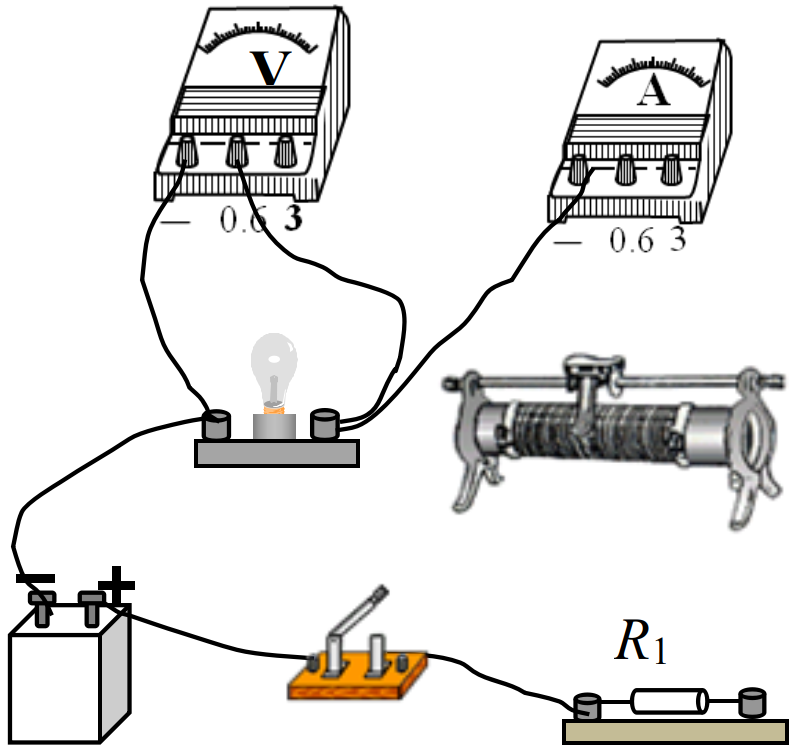
\includegraphics[width=0.7\linewidth]{picture/screenshot066}
\caption{}\label{}
\end{subfigure}
\begin{subfigure}{0.4\linewidth}
\centering
\includesvg[width=0.7\linewidth]{picture/svg/GZ-3-tiyou-1047} 
\caption{}\label{}
\end{subfigure}
\end{figure}




\item 
现有$ 10 \ \Omega $、$ 20 \ \Omega $和$ 50 \ \Omega $的定值电阻,电路中的电阻$ R_{1} $ 应选 \underlinegap $ \Omega $的定值电阻。

\item 
测量结束后,应先断开开关,拆除 \underlinegap 两端的导线,再拆除其他导线,最后整理好器材。

\item 
小明处理数据后将$ P $、$ U_{2} $ 描点在坐标纸上,并作出了一条直线,如题$ 10-2 $ 图所示。 请指出图
象中不恰当的地方。


\end{enumerate}


\tk{
\begin{enumerate}
%\renewcommand{\labelenumi}{\arabic{enumi}.}
% A(\Alph) a(\alph) I(\Roman) i(\roman) 1(\arabic)
%设定全局标号series=example	%引用全局变量resume=example
%[topsep=-0.3em,parsep=-0.3em,itemsep=-0.3em,partopsep=-0.3em]
%可使用leftmargin调整列表环境左边的空白长度 [leftmargin=0em]
\item
如图
\begin{center}
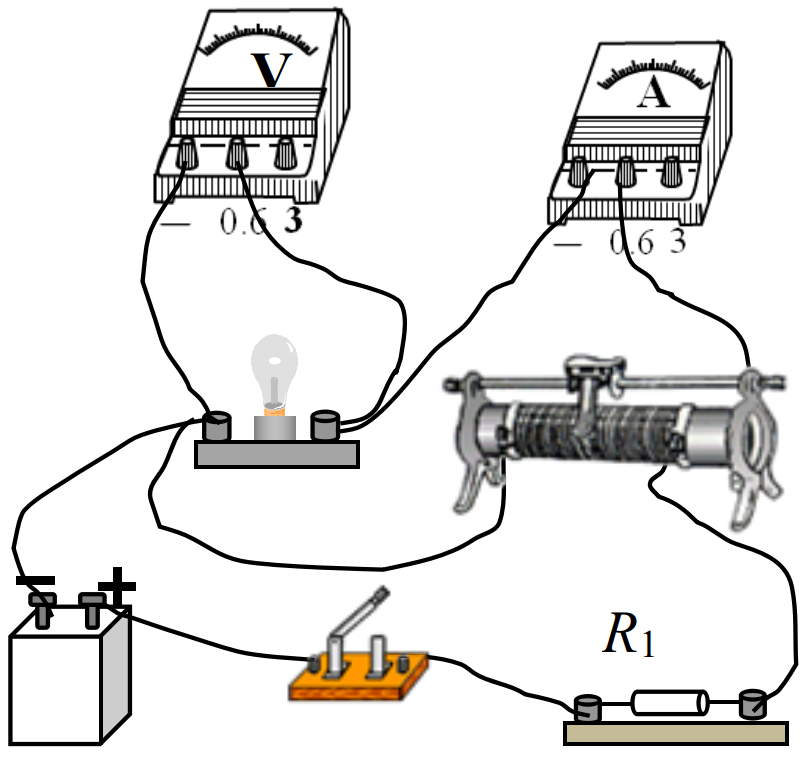
\includegraphics[width=0.7\linewidth]{picture/screenshot067}
\end{center}
\item 
$ 10 $
\item 
电池
\item 
图线不应画为直线;横坐标的标度不恰当.
\end{enumerate}
} 


\item 
\exwhere{$ 2018 $ 年全国卷}
某实验小组利用如图($ a $)所示的电路探究在 $ 25 \ \celsius \sim 80 \ \celsius $ 范围内
某热敏电阻的温度特性。所用器材有:置于温控室(图中虚线区域)中的热敏电阻 $ R_T $,其标称值($ 25 \ \celsius $
时的阻值)为 $ 900.0 \ \Omega $;电源 $ E $( $ 6 \ V $,内阻可忽略);电压表 \voltmetermytikz 
(量程 $ 150 \ m V $ );定值电阻 $ R_{0} $(阻
值 $ 20.0 \ \Omega $ ),滑动变阻器 $ R_{1} $(最大阻值为 $ 1000 \ \Omega $ );电阻箱 $ R_{2} $(阻值范围 $ 0 \sim 999.9 \ \Omega $ );单刀开关
$ S_{1} $,单刀双掷开关 $ S_{2} $。
\begin{figure}[h!]
\centering
\begin{subfigure}{0.4\linewidth}
\centering
\includesvg[width=0.7\linewidth]{picture/svg/GZ-3-tiyou-1048} 
\caption{}\label{}
\end{subfigure}
\begin{subfigure}{0.4\linewidth}
\centering
\includesvg[width=0.7\linewidth]{picture/svg/GZ-3-tiyou-1049} 
\caption{}\label{}
\end{subfigure}
\begin{subfigure}{0.4\linewidth}
\centering
\includesvg[width=0.7\linewidth]{picture/svg/GZ-3-tiyou-1050} 
\caption{}\label{}
\end{subfigure}
\end{figure}



实验时,先按图($ a $)连接好电路,再将温控室的温度 $ t $ 升至
$ 80.0 \ \celsius $。将 $ S_{2} $ 与 $ 1 $ 端接通,闭合 $ S_{1} $,调节 $ R_{1} $ 的滑片位置,使电压表读数为某一值 $ U_{0} $;保持 $ R_{1} $ 的滑
片位置不变,将 $ R_{2} $ 置于最大值,将 $ S_{2} $ 与 $ 2 $ 端接通,调节 $ R_{2} $,使电压表读数仍为 $ U_{0} $;断开 $ S_{1} $,记下
此时 $ R_{2} $ 的读数。逐步降低温控室的温度 $ t $,得到相应温度下 $ R_{2} $ 的阻值,直至温度降到 $ 25.0 \ \celsius $。实验
得到的 $ R_{2} -t $ 数据见下表。
\begin{table}[h!]
\centering 
\begin{tabular}{|l|l|l|l|l|l|l|l|}
\hline$t / \celsius $ & 25.0 & 30.0 & 40.0 & 50.0 & 60.0 & 70.0 & 80.0 \\
\hline$R_{2} / \Omega$ & 900.0 & 680.0 & 500.0 & 390.0 & 320.0 & 270.0 & 240.0 \\
\hline
\end{tabular}
\end{table} 


回答下列问题:
\begin{enumerate}
%\renewcommand{\labelenumi}{\arabic{enumi}.}
% A(\Alph) a(\alph) I(\Roman) i(\roman) 1(\arabic)
%设定全局标号series=example	%引用全局变量resume=example
%[topsep=-0.3em,parsep=-0.3em,itemsep=-0.3em,partopsep=-0.3em]
%可使用leftmargin调整列表环境左边的空白长度 [leftmargin=0em]
\item
在闭合 $ S_{1} $ 前,图($ a $)中 $ R_{1} $ 的滑片应移动到
\underlinegap 
(填“$ a $”或“$ b $”)端;

\item 
在图($ b $)的坐标纸上补齐数据表中所给数据点,并作出 $ R_{2} -t $ 曲线;


\item 
由图($ b $)可得到 $ R_T $ 在 $ 25 \ \celsius \sim 80 \ \celsius $ 范围内的温度特性。当 $ t=44.0 \ \celsius $ 时,可得 $ R_T= $ \underlinegap $ \Omega $;

\item 
将 $ R_T $ 握于手心,手心温度下 $ R_{2} $ 的相应读数如图($ c $)所示,该读数为
为
\underlinegap 
$ \Omega $,
则手心温度
\underlinegap 
$ \celsius $。


\end{enumerate}



\tk{
\begin{enumerate}
%\renewcommand{\labelenumi}{\arabic{enumi}.}
% A(\Alph) a(\alph) I(\Roman) i(\roman) 1(\arabic)
%设定全局标号series=example	%引用全局变量resume=example
%[topsep=-0.3em,parsep=-0.3em,itemsep=-0.3em,partopsep=-0.3em]
%可使用leftmargin调整列表环境左边的空白长度 [leftmargin=0em]
\item
$ b $
\item 
如图
\begin{center}
\includesvg[width=0.23\linewidth]{picture/svg/GZ-3-tiyou-1051} 
\end{center}
\item 
$ 450 $
\item 
$ 620.0 $ \quad $ 33.0 $
\end{enumerate} 
} 



\item 
\exwhere{$ 2013 $ 年山东卷}
霍尔效应是电磁基本现象之一,近期我国科学家在该领域的实
验研究上取得了突破性进展。如图丙所示,在一矩形半导体薄
片的 $ P $、$ Q $ 间通入电流 $ I $,同时外加与薄片垂直的磁场 $ B $,在 $ M $、
$ N $ 间出现电压 $ U_H $,这种现象称为霍尔效应,$ U_H $ 为霍尔电压,
且满足$U_{H}=k \frac{I B}{d}$,式中 $ d $ 为薄片的厚度,$ k $ 为霍尔系数。某
同学通过实验测定该半导体薄片的霍尔系数。
\begin{figure}[h!]
\centering
\begin{subfigure}{0.4\linewidth}
\centering
\includesvg[width=0.7\linewidth]{picture/svg/GZ-3-tiyou-1054} 
\caption{}\label{}
\end{subfigure}
\begin{subfigure}{0.4\linewidth}
\centering
\includesvg[width=0.7\linewidth]{picture/svg/GZ-3-tiyou-1053} 
\caption{}\label{}
\end{subfigure}

\end{figure}


\begin{enumerate}
%\renewcommand{\labelenumi}{\arabic{enumi}.}
% A(\Alph) a(\alph) I(\Roman) i(\roman) 1(\arabic)
%设定全局标号series=example	%引用全局变量resume=example
%[topsep=-0.3em,parsep=-0.3em,itemsep=-0.3em,partopsep=-0.3em]
%可使用leftmargin调整列表环境左边的空白长度 [leftmargin=0em]
\item
若该半导体材料是空穴(可视为带正电粒子)导电,电流与磁场方向如图丙所示,该同学用电压
表测量 $ U_H $ 时,应将电压表的“$ + $”接线柱与 \underlinegap (填“$ M $”或“$ N $”)端通过导线连接。


\item 
已知薄片厚度 $ d=0.40 \ mm $。该同学保持磁感应强度 $ B=0.10 \ T $ 不变,改变电流 $ I $ 的大小,测量相应
的 $ U_H $ 值,记录数据如下表所示。
\begin{table}[h!]
\centering 
\begin{tabular}{|l|l|l|l|l|l|l|}
\hline$I\left(\times 10^{-3} A\right)$ & 3.0 & 6.0 & 9.0 & 12.0 & 15.0 & 18.0 \\
\hline$U_{H}\left(\times 10^{-3} V\right)$ & 1.1 & 1.9 & 3.4 & 4.5 & 6.2 & 6.8 \\
\hline
\end{tabular}
\end{table} 


根据表中数据在给定坐标纸上(见答题卡)画出 $ U_H - I $ 图线,利用图线求出该材料的霍尔系数为 \underlinegap 
$ 10-3 \ V \cdot m \cdot A^{-1} \cdot T^{-1} $ (保留 $ 2 $ 位有效数字)。


\item 
该同学查阅资料发现,使半导体薄片中的电流反向再次测量,
取两个方向的测量的平均值,可以减小霍尔系数的测量误差,为
此该同学设计了如图丁所示的测量电路。$ S_{1} $、$ S_{2} $ 均为单刀双掷开
关,虚线框内为半导体薄片(未画出)。为使电流自 $ Q $ 端流入,$ P $
端流出,应将 $ S_{1} $ 掷向 \underlinegap (填“$ a $”或“$ b $”), $ S_{2} $ 掷向 \underlinegap (填“$ c $”
或“$ d $”)。



为了保证测量安全,该同学改进了测量电路,将一合适的定值电阻串联在电路中。在保持其它
连接不变的情况下,该定值电阻串接在相邻器件 \underlinegap 与 \underlinegap (填器件代号)之间。


\end{enumerate}


\tk{
\begin{enumerate}
%\renewcommand{\labelenumi}{\arabic{enumi}.}
% A(\Alph) a(\alph) I(\Roman) i(\roman) 1(\arabic)
%设定全局标号series=example	%引用全局变量resume=example
%[topsep=-0.3em,parsep=-0.3em,itemsep=-0.3em,partopsep=-0.3em]
%可使用leftmargin调整列表环境左边的空白长度 [leftmargin=0em]
\item
$ M $
\item 
如图所示 \quad $ 1.5 $($ 1.4 $ 或 $ 1.6 $)
\begin{center}
 \includesvg[width=0.23\linewidth]{picture/svg/GZ-3-tiyou-1055} 
\end{center}
\item 
$ b $ \quad $ c $ \quad $ S_{1} $,$ E $(或 $ S_{2} $,$ E $)
\end{enumerate}
} 


\item 
\exwhere{$ 2013 $ 年广东卷}
图 $ 17 $($ a $)是测量电阻 $ RX $ 的原理图。学生电源
输出电压可调,电流表量程选 $ 0.6 \ A $(内阻不计),标有
长度刻度的均匀电阻丝 $ ab $ 的总长为 $ 30.0 \ cm $。
\begin{figure}[h!]
\centering
\begin{subfigure}{0.4\linewidth}
\centering
\includesvg[width=0.7\linewidth]{picture/svg/GZ-3-tiyou-1057} 
\caption{}\label{}
\end{subfigure}
\begin{subfigure}{0.4\linewidth}
\centering
\includesvg[width=0.7\linewidth]{picture/svg/GZ-3-tiyou-1058} 
\caption{}\label{}
\end{subfigure}
\begin{subfigure}{0.4\linewidth}
\centering
\includesvg[width=0.7\linewidth]{picture/svg/GZ-3-tiyou-1059} 
\caption{}\label{}
\end{subfigure}
\end{figure}

\begin{enumerate}
%\renewcommand{\labelenumi}{\arabic{enumi}.}
% A(\Alph) a(\alph) I(\Roman) i(\roman) 1(\arabic)
%设定全局标号series=example	%引用全局变量resume=example
%[topsep=-0.3em,parsep=-0.3em,itemsep=-0.3em,partopsep=-0.3em]
%可使用leftmargin调整列表环境左边的空白长度 [leftmargin=0em]
\item
根
据原理图连接图$ 17 $($ b $)的实物图。


\item 
断开 $ S_{2} $,合上 $ S_{1} $;调节电源输出电压为 $ 3.0 \ V $ 时,单位长度电阻丝的电压 $ u= $
\underlinegap 
$ V/cm $,
记录此时电流表 $ A_{1} $ 的示数。


\item 
保持 $ S_{1} $ 闭合,合上 $ S_{2} $;滑动 $ c $ 点改变 $ ac $ 的长度 $ L $,同时调节电源输出电压,使电流表 $ A_{1} $ 的示数
与步骤②记录的值相同,记录长度 $ L $ 和 $ A_{2} $ 的示数 $ I $。测量 $ 6 $ 组 $ L $ 和 $ I $ 值,测量数据已在图 $ 17 $($ c $)
中标出,写出 $ R_X $ 与 $ L $、$ I $、$ u $ 的关系式 $ R_X= $
\underlinegap 
;根据图 $ 17 $($ c $)用作图法算出
$ R_X= $ \underlinegap 
$ \Omega $。

\end{enumerate}


\tk{
\begin{enumerate}
%\renewcommand{\labelenumi}{\arabic{enumi}.}
% A(\Alph) a(\alph) I(\Roman) i(\roman) 1(\arabic)
%设定全局标号series=example	%引用全局变量resume=example
%[topsep=-0.3em,parsep=-0.3em,itemsep=-0.3em,partopsep=-0.3em]
%可使用leftmargin调整列表环境左边的空白长度 [leftmargin=0em]
\item
如图所示
\begin{center}
\includesvg[width=0.23\linewidth]{picture/svg/GZ-3-tiyou-1060} 	
\end{center}
\item 	
$ 0.10 $
\item 
$R_{x}=\frac{L u}{I}$ \quad $R_{x}=k u=6.0 \ \Omega$
\end{enumerate}
} 


\item 
\exwhere{$ 2012 $ 年理综新课标卷}
图中虚线框内存在一沿水平方向、且与纸面垂直的匀强磁场。现通过测量通电导线在磁场中所
受的安培力,来测量磁场的磁感应强度大小、并
判定其方向。所用部分器材已在图中给出,其中 $ D $
为位于纸面内的 $ U $ 形金属框,其底边水平,两侧
边竖直且等长;$ E $ 为直流电源;$ R $ 为电阻箱; \ammetermytikz 为
电流表;$ S $ 为开关。此外还有细沙、天平、米尺和
若干轻质导线。
\begin{figure}[h!]
\centering
\includesvg[width=0.43\linewidth]{picture/svg/GZ-3-tiyou-1061} 
\end{figure}

\begin{enumerate}
%\renewcommand{\labelenumi}{\arabic{enumi}.}
% A(\Alph) a(\alph) I(\Roman) i(\roman) 1(\arabic)
%设定全局标号series=example	%引用全局变量resume=example
%[topsep=-0.3em,parsep=-0.3em,itemsep=-0.3em,partopsep=-0.3em]
%可使用leftmargin调整列表环境左边的空白长度 [leftmargin=0em]
\item
在图中画线连接成实验电路图。
\item 
完成下列主要实验步骤中的填空。
\begin{enumerate}
%\renewcommand{\labelenumi}{\arabic{enumi}.}
% A(\Alph) a(\alph) I(\Roman) i(\roman) 1(\arabic)
%设定全局标号series=example	%引用全局变量resume=example
%[topsep=-0.3em,parsep=-0.3em,itemsep=-0.3em,partopsep=-0.3em]
%可使用leftmargin调整列表环境左边的空白长度 [leftmargin=0em]
\item
按图接线。

\item 
保持开关 $ S $ 断开,在托盘内加入适量细沙,使 $ D $ 处于平衡状态;然后用天平称出细沙质量 $ m_{1} $。

\item 
闭合开关 $ S $,调节 $ R $ 的值使电流大小适当,在托盘内重新加入适量细沙,使 $ D $ \underlinegap ;然后读
出 \underlinegap ,并用天平称出 \underlinegap 。



\item 
用米尺测量。


\end{enumerate}


\item 
用测量的物理量和重力加速度 $ g $ 表示磁感应强度的大小,可以得出 $ B= $ \underlinegap 。
\item 
判定磁感应强度方向的方法是:若 \underlinegap ,磁感应强度方向垂直纸面向外;反之,磁
感应强度方向垂直纸面向里。

\end{enumerate}

\tk{
\begin{enumerate}
%\renewcommand{\labelenumi}{\arabic{enumi}.}
% A(\Alph) a(\alph) I(\Roman) i(\roman) 1(\arabic)
%设定全局标号series=example	%引用全局变量resume=example
%[topsep=-0.3em,parsep=-0.3em,itemsep=-0.3em,partopsep=-0.3em]
%可使用leftmargin调整列表环境左边的空白长度 [leftmargin=0em]
\item
连线如图示
\begin{center}
\includesvg[width=0.23\linewidth]{picture/svg/GZ-3-tiyou-1062} 
\end{center}
\item 
\begin{enumerate}
%\renewcommand{\labelenumi}{\arabic{enumi}.}
% A(\Alph) a(\alph) I(\Roman) i(\roman) 1(\arabic)
%设定全局标号series=example	%引用全局变量resume=example
%[topsep=-0.3em,parsep=-0.3em,itemsep=-0.3em,partopsep=-0.3em]
%可使用leftmargin调整列表环境左边的空白长度 [leftmargin=0em]
\item none
\item none
\item 
重新处于平衡状态\\
电流表的示数 $ I $\\
此时细沙的质量 $ m_{2} $
\item 
$ D $ 的底边长 $ L $
\end{enumerate}
\item 
$B=\frac{\left|m_{1}-m_{2}\right| g}{I L}$
\item 
$m_{2}>m_{1}$
\end{enumerate}
} 





\item
\exwhere{$ 2011 $ 年理综山东卷}
某同学利用图甲所示电路,探究了电源在不同负载下的输出功率。
\begin{figure}[h!]
\centering
\includesvg[width=0.23\linewidth]{picture/svg/GZ-3-tiyou-1063}
\end{figure}

\begin{enumerate}
%\renewcommand{\labelenumi}{\arabic{enumi}.}
% A(\Alph) a(\alph) I(\Roman) i(\roman) 1(\arabic)
%设定全局标号series=example	%引用全局变量resume=example
%[topsep=-0.3em,parsep=-0.3em,itemsep=-0.3em,partopsep=-0.3em]
%可使用leftmargin调整列表环境左边的空白长度 [leftmargin=0em]
\item
所得实验数据如下表,请在给出的直角坐标系上画出 $ U-I $ 图像。
\begin{table}[h!]
\centering 
\begin{tabular}{|c|c|c|c|c|c|c|}
\hline 
$ U/V $ & 1.96 & 1.86 & 1.80 & 1.84 & 1.64 & 1.56
 \\
\hline
$ I/A $ & 0.05 & 0.15 & 0.25 & 0.35 & 0.45 & 0.55\\ 
\hline 
\end{tabular}
\end{table} 
\begin{figure}[h!]
\centering
\includesvg[width=0.43\linewidth]{picture/svg/GZ-3-tiyou-1064}
\end{figure}




\item 
根据所画 $ U-I $ 图像,可求得电流 $ I=0.20 \ A $ 时电源的输出功率为
\underlinegap 
$ W $。(保留两位有效数)




\item 
实验完成后,该同学对实验方案进行了反思,认为按图甲电路
进行实验操作的过程中存在安全隐患,并对电路重新设计。在图
乙所示的电路中,你认为既能测出电源在不同负载下的输出功
率,又能消除安全隐患的是 \underlinegap 。($ R_{x} $阻值未知)
\pfourchoices
{\includesvg[width=4.3cm]{picture/svg/GZ-3-tiyou-1065}}
{\includesvg[width=4.3cm]{picture/svg/GZ-3-tiyou-1066}}
{\includesvg[width=4.3cm]{picture/svg/GZ-3-tiyou-1067}}
{\includesvg[width=4.3cm]{picture/svg/GZ-3-tiyou-1068}}





\end{enumerate}



\tk{
\begin{enumerate}
%\renewcommand{\labelenumi}{\arabic{enumi}.}
% A(\Alph) a(\alph) I(\Roman) i(\roman) 1(\arabic)
%设定全局标号series=example	%引用全局变量resume=example
%[topsep=-0.3em,parsep=-0.3em,itemsep=-0.3em,partopsep=-0.3em]
%可使用leftmargin调整列表环境左边的空白长度 [leftmargin=0em]
\item
如图所示
\begin{center}
\includesvg[width=0.23\linewidth]{picture/svg/GZ-3-tiyou-1069} 
\end{center}
\item 
$ 0.37 $(或 $ 0.36 $)
\item 
BC
\end{enumerate}
} 


\item 
\exwhere{$ 2011 $ 年物理江苏卷}
某同学利用如图所示的实验电路来测量电阻的阻值。
\begin{figure}[h!]
\centering
\includesvg[width=0.23\linewidth]{picture/svg/GZ-3-tiyou-1070}
\end{figure}


\begin{enumerate}
%\renewcommand{\labelenumi}{\arabic{enumi}.}
% A(\Alph) a(\alph) I(\Roman) i(\roman) 1(\arabic)
%设定全局标号series=example	%引用全局变量resume=example
%[topsep=-0.3em,parsep=-0.3em,itemsep=-0.3em,partopsep=-0.3em]
%可使用leftmargin调整列表环境左边的空白长度 [leftmargin=0em]
\item
将电阻箱接入 $ a $、$ b $ 之间,闭合开关。适当调节滑动变阻器 $ R ^{\prime} $后保持其
阻值不变。改变电阻箱的阻值 $ R $,得到一组电压表的示数 $ U $ 与 $ R $ 的数据
如下表:
\begin{table}[h!]
\centering 
\begin{tabular}{|c|c|c|c|c|c|c|}
\hline 
电阻$ R/ \Omega $ & $ 5.0 $ & $ 10.0 $ & $ 15.0 $ & $ 25.0 $ & $ 35.0 $ & $ 45.0 $
 \\
\hline
电压$ U/V $ & $ 1.00 $ & $ 1.50 $ & $ 1.80 $ & $ 2.14 $ & $ 2.32 $ & $ 2.45 $\\ 
\hline 
\end{tabular}
\end{table} 
请根据实验数据作出 $ U-R $ 关系图象。
\begin{figure}[h!]
\centering
\includesvg[width=0.23\linewidth]{picture/svg/GZ-3-tiyou-1071}
\end{figure}




\item 
用待测电阻 $ R_{x} $ 替换电阻箱,读得电压表示数为 $ 2.00 \ V $。利用 (1) 中测
绘的 $ U-R $ 图象可得 $ R_{x} =$ \underlinegap $ \Omega $。


\item 
使用较长时间后,电池的电动势可认为不变,但内阻增大。若仍
用本实验装置和⑴中测绘的 $ U-R $ 图象测定某一电阻,则测定结果
将 \underlinegap (选填“偏大”或“偏小”)。现将一已知阻值为 $ 10 \ \Omega $的电
阻换接在 $ a $、$ b $ 之间,你应如何调节滑动变阻器,便仍可利用本实
验装置和 (1) 中测绘的 $ U-R $ 图象实现对待测电阻的准确测定?

\hfullline 


\end{enumerate}


\tk{
\begin{enumerate}
%\renewcommand{\labelenumi}{\arabic{enumi}.}
% A(\Alph) a(\alph) I(\Roman) i(\roman) 1(\arabic)
%设定全局标号series=example	%引用全局变量resume=example
%[topsep=-0.3em,parsep=-0.3em,itemsep=-0.3em,partopsep=-0.3em]
%可使用leftmargin调整列表环境左边的空白长度 [leftmargin=0em]
\item
如图
\begin{center}
\includesvg[width=0.23\linewidth]{picture/svg/GZ-3-tiyou-1072} 
\end{center}
\item 	
$ 20 $($ 19 \sim 21 $ 都算对)	
\item 
偏小\\
改变滑动变阻器阻值,使电压表示数为$ 1.50 \ V $
\end{enumerate}
} 


\item 
\exwhere{$ 2014 $ 年理综广东卷}
某同学设计的可调电源电路如图 $ (a) $所示,$ R_{0} $ 为保护电阻,$ P $ 为滑动变阻器的滑片,闭
合电键 $ S $。
\begin{figure}[h!]
\centering
\begin{subfigure}{0.4\linewidth}
\centering
\includesvg[width=0.7\linewidth]{picture/svg/GZ-3-tiyou-1073} 
\caption{}\label{}
\end{subfigure}
\begin{subfigure}{0.4\linewidth}
\centering
\includesvg[width=0.7\linewidth]{picture/svg/GZ-3-tiyou-1074} 
\caption{}\label{}
\end{subfigure}
\end{figure}

\begin{enumerate}
%\renewcommand{\labelenumi}{\arabic{enumi}.}
% A(\Alph) a(\alph) I(\Roman) i(\roman) 1(\arabic)
%设定全局标号series=example	%引用全局变量resume=example
%[topsep=-0.3em,parsep=-0.3em,itemsep=-0.3em,partopsep=-0.3em]
%可使用leftmargin调整列表环境左边的空白长度 [leftmargin=0em]
\item
用电压表测量 $ A $、$ B $ 两端的电压;将电压表调零,选择 $ 0-3 \ V $ 档,示数如图 $ 22(b) $,电压值为
\underlinegap 
$ V $。

\item 
在接通外电路之前,为了保证外电路的安全,滑片$ P $应先置于
\underlinegap 
端。

\item 
要使输出电压 $ U $ 变大,滑片 $ P $ 应向 \underlinegap 端。



\item 
若电源电路中不接入 $ R_{0} $,则在使用过程中,存在 \underlinegap 
的风险(填“断路”或“短路”)。

\end{enumerate}



\tk{
\begin{enumerate}
%\renewcommand{\labelenumi}{\arabic{enumi}.}
% A(\Alph) a(\alph) I(\Roman) i(\roman) 1(\arabic)
%设定全局标号series=example	%引用全局变量resume=example
%[topsep=-0.3em,parsep=-0.3em,itemsep=-0.3em,partopsep=-0.3em]
%可使用leftmargin调整列表环境左边的空白长度 [leftmargin=0em]
\item
$ 1.30 $
\item 
A
\item 
B
\item 
短路
\end{enumerate}
} 

\item 
\exwhere{$ 2015 $ 年理综重庆卷}
同学们测量某电阻丝的电阻 $ R_{x} $,所用电流表的内阻与 $ R_{x} $ 相当,电压表
可视为理想电压表。
\begin{figure}[h!]
\centering
\begin{subfigure}{0.4\linewidth}
\centering
\includesvg[width=0.7\linewidth]{picture/svg/GZ-3-tiyou-1075} 
\caption{}\label{}
\end{subfigure}
\begin{subfigure}{0.4\linewidth}
\centering
\includesvg[width=0.7\linewidth]{picture/svg/GZ-3-tiyou-1076} 
\caption{}\label{}
\end{subfigure}
\begin{subfigure}{0.4\linewidth}
\centering
\includesvg[width=0.7\linewidth]{picture/svg/GZ-3-tiyou-1077} 
\caption{}\label{}
\end{subfigure}
\begin{subfigure}{0.4\linewidth}
\centering
\includesvg[width=0.7\linewidth]{picture/svg/GZ-3-tiyou-1078} 
\caption{}\label{}
\end{subfigure}
\end{figure}


\begin{enumerate}
%\renewcommand{\labelenumi}{\arabic{enumi}.}
% A(\Alph) a(\alph) I(\Roman) i(\roman) 1(\arabic)
%设定全局标号series=example	%引用全局变量resume=example
%[topsep=-0.3em,parsep=-0.3em,itemsep=-0.3em,partopsep=-0.3em]
%可使用leftmargin调整列表环境左边的空白长度 [leftmargin=0em]
\item
若使用图 $ a $ 所示电路图进行实验,要使得 $ R_{x} $ 的测量值更接近
真实值,电压表的 $ a $ 端应连接到电路的
\underlinegap 
点(选填“$ b $”或“$ c $”)。



\item 
测得电阻丝的 $ U-I $ 图如图 $ b $ 所示,则 $ R_{x} $ 为
\underlinegap 
$ \Omega $(保
留两位有效数字)。



\item 
实验中,随电压进一步增加电阻丝逐渐进入炽热状态。某同学发
现对炽热电阻丝吹气,其阻值会变化。他们对此现象进行探究,在控制电阻丝两端的电压为 $ 10 \ V $ 的
条件下,得到电阻丝的电阻 $ R_{x} $ 随风速 $ v $ (用风速计测)的变化关系如图 $ c $ 所示。由图可知当风
速增加时,$ R_{x} $ 会
\underlinegap 
(选填“增大”或“减小”)。当风速增加过程中,为保持电阻丝两端电压为
$ 10 \ V $,需要将滑动变阻器 $ R_W $ 的滑片向
\underlinegap 
端调节(选填“$ M $”或“$ N $”)。

\item 
为了通过电压表的示数来显示风速,同学们设计了如图 $ d $ 所示的电路。其中 $ R $ 为两只阻值相
同的电阻,$ R_{x} $ 为两根相同的电阻丝,一根置于气流中,另一根不受气流影响,$ V $ 为待接入的理想电
压表。如果要求在测量中,风速从零开始增加,电压表的示数也从零开始增加,则电压表的“$ + $”端
和“$ - $”端应分别连接到电路中的
\underlinegap 
点和
\underlinegap 
点(在“$ a $”“$ b $”“$ c $”“$ d $”中选填)。	
\end{enumerate}


\tk{
\begin{enumerate}
%\renewcommand{\labelenumi}{\arabic{enumi}.}
% A(\Alph) a(\alph) I(\Roman) i(\roman) 1(\arabic)
%设定全局标号series=example	%引用全局变量resume=example
%[topsep=-0.3em,parsep=-0.3em,itemsep=-0.3em,partopsep=-0.3em]
%可使用leftmargin调整列表环境左边的空白长度 [leftmargin=0em]
\item
$ c $
\item 
$ 4.1 $ ($ 4.0 \sim 4.2 $)
\item 
减小 \quad $ M $
\item 
$ b $ \quad $ d $
\end{enumerate}
} 


\item 
\exwhere{$ 2015 $ 年海南卷}
某同学利用图($ a $)所示电路测量电容器充电时两极板间的电压随时间的变化。
实验中使用的器材为:电池 $ E $(内阻很小)、开关 $ S_{1} $ 和 $ S_{2} $、电容器 $ C $(约 $ 100 \mu F $)、电阻 $ R_{1} $(
约 $ 200 \ k\Omega $)、
电阻 $ R_{2} $($ 1 \ k\Omega $)、电压表 $ V $(量程 $ 6 \ V $)、秒表、导线若干。
\begin{figure}[h!]
\centering
\begin{subfigure}{0.4\linewidth}
\centering
\includesvg[width=0.7\linewidth]{picture/svg/GZ-3-tiyou-1079} 
\caption{}\label{}
\end{subfigure}
\begin{subfigure}{0.4\linewidth}
\centering
\includesvg[width=0.7\linewidth]{picture/svg/GZ-3-tiyou-1080} 
\caption{}\label{}
\end{subfigure}
\begin{subfigure}{0.4\linewidth}
\centering
\includesvg[width=0.7\linewidth]{picture/svg/GZ-3-tiyou-1081} 
\caption{}\label{}
\end{subfigure}
\end{figure}

\begin{enumerate}
%\renewcommand{\labelenumi}{\arabic{enumi}.}
% A(\Alph) a(\alph) I(\Roman) i(\roman) 1(\arabic)
%设定全局标号series=example	%引用全局变量resume=example
%[topsep=-0.3em,parsep=-0.3em,itemsep=-0.3em,partopsep=-0.3em]
%可使用leftmargin调整列表环境左边的空白长度 [leftmargin=0em]
\item
按 图($ a $)所示的电路原理图将图($ b $)中实物图连线。

\item 
先闭合开关 $ S_{2} $,再断开开关 $ S_{2} $;闭合开关 $ S_{1} $,同时按下秒表开始计时。若某时刻电压表示数如
图($ c $)所示,电压表的读数为 \underlinegap $ V $(保留 $ 2 $ 位小数)。

\item 
该同学每隔 $ 10 \ s $ 记录一次电压表的读数 $ U $,记录的数据
如下表所示,在答题卡给出的坐标纸上绘出 $ U-I $ 图线。已知
只有一个数据点误差较大,该数据点对应的表中的时间是
\underlinegap 
$ s $。
\begin{table}[h!]
\centering 
\begin{tabular}{|c|c|c|c|c|c|c|}
\hline 
时间$ t/s $ & $ 10.0 $ & $ 20.0 $ & $ 30.0 $ & $ 40.0 $ & $ 50.0 $ & $ 60.0 $
 \\
\hline
电压$ U/V $ & $ 2.14 $ & $ 3.45 $ & $ 4.23 $ & $ 4.51 $ & $ 5.00 $ & $ 5.18 $\\ 
\hline 
\end{tabular}
\end{table} 
\begin{figure}[h!]
\centering
\includesvg[width=0.23\linewidth]{picture/svg/GZ-3-tiyou-1082}
\end{figure}





\item 
电路中 $ C $、$ R_{2} $ 和 $ S_{2} $ 构成的回路的作用是 \hfullline 。


\end{enumerate}

\tk{
\begin{enumerate}
%\renewcommand{\labelenumi}{\arabic{enumi}.}
% A(\Alph) a(\alph) I(\Roman) i(\roman) 1(\arabic)
%设定全局标号series=example	%引用全局变量resume=example
%[topsep=-0.3em,parsep=-0.3em,itemsep=-0.3em,partopsep=-0.3em]
%可使用leftmargin调整列表环境左边的空白长度 [leftmargin=0em]
\item
如答图示
\begin{center}
\heiti 
 \includesvg[width=0.23\linewidth]{picture/svg/GZ-3-tiyou-1084} 
\end{center}
\item 
$ 3.6 \ V $
\item 
$ U-I $图像如图 \quad $ 40 \ s $
 	\begin{center}
\includesvg[width=0.23\linewidth]{picture/svg/GZ-3-tiyou-1083} 
\end{center}
\item 
使实验前电容器两极板上的电荷相中和
\end{enumerate}
} 




\item
\exwhere{$ 2016 $ 年新课标 \lmd{1} 卷}
现要组装一个由热敏电阻控制的报警系统,要求当热敏电阻的
温度达到或超过 $ 60 \ \celsius $ 时,系统报警。提供的器材有:热敏电阻,报警器(内阻很小,流过的电流
超过 $ I_{c} $ 时就会报警),电阻箱(最大阻值为 $ 999.9 \ \Omega $ ),直流电源(输出电压为 $ U $,内阻不计),
滑动变阻器 $ R_{1} $ (最大阻值为 $ 1000 \ \Omega $ ),滑动变阻器 $ R_{2} $ (最大阻值为 $ 2000 \ \Omega $ ),单刀双掷开关一个,
导线若干。
\begin{figure}[h!]
\centering
\includesvg[width=0.43\linewidth]{picture/svg/GZ-3-tiyou-1085}
\end{figure}

在室温下对系统进行调节。已知 $ U $ 约为 $ 18 \ V $, $ I_{c} $ 约为 $ 10 \ mA $;
流过报警器的电流超过 $ 20 \ mA $ 时,报警器可能损坏;该热敏
电阻的阻值随温度升高而减小,在 $ 60 \ \celsius $ 时阻值为 $ 650.0 \ \Omega $。

\begin{enumerate}
%\renewcommand{\labelenumi}{\arabic{enumi}.}
% A(\Alph) a(\alph) I(\Roman) i(\roman) 1(\arabic)
%设定全局标号series=example	%引用全局变量resume=example
%[topsep=-0.3em,parsep=-0.3em,itemsep=-0.3em,partopsep=-0.3em]
%可使用leftmargin调整列表环境左边的空白长度 [leftmargin=0em]
\item
在答题卡上完成待调节的报警系统原理电路图的连线。

\item 
电路中应选用滑动变阻器 \underlinegap (填“ $ R_{1} $ ”或
“ $ R_{2} $ ”)。

\item 
按照下列步骤调节此报警系统:
\begin{enumerate}
%\renewcommand{\labelenumi}{\arabic{enumi}.}
% A(\Alph) a(\alph) I(\Roman) i(\roman) 1(\arabic)
%设定全局标号series=example	%引用全局变量resume=example
%[topsep=-0.3em,parsep=-0.3em,itemsep=-0.3em,partopsep=-0.3em]
%可使用leftmargin调整列表环境左边的空白长度 [leftmargin=0em]
\item
电路接通前,需将电阻箱调到一固定的阻值,根据实验要
求,这一阻值为 \underlinegap $ \Omega $;滑动变阻器的滑片应置于 \underlinegap (填“$ a $”或“$ b $”)端附近,不能置于另一
端的原因是 \hfullline 。


\item 
将开关向 \underlinegap (填“$ c $”或“$ d $”)端闭合,缓慢移动滑动变阻器的滑片,直至 \hfullline 
。

\end{enumerate}


\item 
保持滑动变阻器滑片的位置不变,将开关向另一端闭合,报警系统即可正常使用。




\end{enumerate}


\tk{
\begin{enumerate}
%\renewcommand{\labelenumi}{\arabic{enumi}.}
% A(\Alph) a(\alph) I(\Roman) i(\roman) 1(\arabic)
%设定全局标号series=example	%引用全局变量resume=example
%[topsep=-0.3em,parsep=-0.3em,itemsep=-0.3em,partopsep=-0.3em]
%可使用leftmargin调整列表环境左边的空白长度 [leftmargin=0em]
\item
如下图
\begin{center}
 \includesvg[width=0.23\linewidth]{picture/svg/GZ-3-tiyou-1086} 
\end{center}
\item 
$ R_{2} $
\item 
\begin{enumerate}
%\renewcommand{\labelenumi}{\arabic{enumi}.}
% A(\Alph) a(\alph) I(\Roman) i(\roman) 1(\arabic)
%设定全局标号series=example	%引用全局变量resume=example
%[topsep=-0.3em,parsep=-0.3em,itemsep=-0.3em,partopsep=-0.3em]
%可使用leftmargin调整列表环境左边的空白长度 [leftmargin=0em]
\item
$ 650.0 $
\item 
$ b $\\
 接通电源后,流过报警器的电流会超过 $ 20 \ mA $,报警器可能损坏坏
 \item 
 $ c $ \quad 报警器开始报警
\end{enumerate}
\end{enumerate}
} 


\item 
\exwhere{$ 2016 $ 年新课标 \lmd{3} 卷}
某同学用图中所给器材进行与安培力有关的实验。两根金属导轨
$ ab $ 和 $ a_{1} b_{1} $ 固定在同一水平面内且相互平行,足够大的电磁铁(未画出)的 $ N $ 极位于两导轨的正上方,
$ S $ 极位于两导轨的正下方,一金属棒置于导轨上且两导
轨垂直。
\begin{figure}[h!]
\centering
\includesvg[width=0.23\linewidth]{picture/svg/GZ-3-tiyou-1087}
\end{figure}

\begin{enumerate}
%\renewcommand{\labelenumi}{\arabic{enumi}.}
% A(\Alph) a(\alph) I(\Roman) i(\roman) 1(\arabic)
%设定全局标号series=example	%引用全局变量resume=example
%[topsep=-0.3em,parsep=-0.3em,itemsep=-0.3em,partopsep=-0.3em]
%可使用leftmargin调整列表环境左边的空白长度 [leftmargin=0em]
\item
在图中画出连线,完成实验电路。要求滑动变阻
器以限流方式接入电路,且在开关闭合后,金属棒沿箭
头所示的方向移动。


\item 
为使金属棒在离开导轨时具有更大的速度,有人
提出以下建议:
\threechoices
{适当增加两导轨间的距离}
{换一根更长的金属棒}
{适当增大金属棒中的电流}

其中正确的是 \underlinegap (填入正确选项前的标号)。





\end{enumerate}

\tk{
\begin{enumerate}
%\renewcommand{\labelenumi}{\arabic{enumi}.}
% A(\Alph) a(\alph) I(\Roman) i(\roman) 1(\arabic)
%设定全局标号series=example	%引用全局变量resume=example
%[topsep=-0.3em,parsep=-0.3em,itemsep=-0.3em,partopsep=-0.3em]
%可使用leftmargin调整列表环境左边的空白长度 [leftmargin=0em]
\item
如图所示
\begin{center}
\includesvg[width=0.23\linewidth]{picture/svg/GZ-3-tiyou-1088} 
\end{center}
\item 
AC
\end{enumerate}
} 


\item 
\exwhere{$ 2016 $ 年江苏卷}
小明同学通过实验探究某一金属电阻的阻值 $ R $ 随温度 $ t $ 的变化关系。已知该
金属电阻在常温下的阻值约 $ 10 \ \Omega $,$ R $ 随 $ t $ 的升高而增大。实验电路如图所示,控温箱用以调节金属
电阻的温度。
\begin{figure}[h!]
\centering
\includesvg[width=0.43\linewidth]{picture/svg/GZ-3-tiyou-1089}
\end{figure}



实验时闭合 $ S $,先将开关 $ K $ 与 $ 1 $ 端闭合,调节金属电
阻的温度,分别记下温度 $ t_{1} $,$ t_{2} $,$ \cdots $和电流表的相应示
数 $ I_{1} $,$ I_{2} $,$ \cdots $.然后将开关 $ K $ 与 $ 2 $ 端闭合,调节电阻箱
使电流表的示数再次为 $ I_{1} $,$ I_{2} $,$ \cdots $,分别记下电阻箱
相应的示数 $ R_{1} $,$ R_{2} $,$ \cdots $。

\begin{enumerate}
%\renewcommand{\labelenumi}{\arabic{enumi}.}
% A(\Alph) a(\alph) I(\Roman) i(\roman) 1(\arabic)
%设定全局标号series=example	%引用全局变量resume=example
%[topsep=-0.3em,parsep=-0.3em,itemsep=-0.3em,partopsep=-0.3em]
%可使用leftmargin调整列表环境左边的空白长度 [leftmargin=0em]
\item
有以下两种电流表,实验电路中应选用 \underlinegap 。


\twochoices
{量程 $ 0 \sim 100 \ mA $,内阻约 $ 2 \ \Omega $}
{量程 $ 0 \sim 0.6 \ A $,内阻可忽略}

\item 
实验过程中,要将电阻箱的阻值由 $ 9.9 \ \Omega $调节至 $ 10.0 \ \Omega $,需
旋转图中电阻箱的旋钮“$ a $”“$ b $”“$ c $”,正确的操作顺序是 \underlinegap 
。

①将旋钮 $ a $ 由“$ 0 $”旋转至“$ 1 $”

②将旋钮 $ b $ 由“$ 9 $”旋转至“$ 0 $”

③将旋钮 $ c $ 由“$ 9 $”旋转至“$ 0 $”



\item 
实验记录的 $ t $ 和 $ R $ 的数据见下表:
\begin{table}[h!]
\centering 
\begin{tabular}{|c|c|c|c|c|c|}
\hline 
温度$ t( \celsius ) $& 20.0 & 40.0 & 60.0 & 80.0 & 100.0
 \\
\hline
阻值$ R( \Omega ) $& 9.6 & 10.4 & 11.1 & 12.1 & 12.8\\ 
\hline 
\end{tabular}
\end{table} 



请根据表中数据,在方格纸上作出 $ R-t $ 图线。
\begin{figure}[h!]
\centering
\includesvg[width=0.23\linewidth]{picture/svg/GZ-3-tiyou-1090}
\end{figure}

由图线求得 $ R $ 随 $ t $ 的变化关系为 $ R= $ \underlinegap $\Omega $。

\end{enumerate}


\tk{
\begin{enumerate}
%\renewcommand{\labelenumi}{\arabic{enumi}.}
% A(\Alph) a(\alph) I(\Roman) i(\roman) 1(\arabic)
%设定全局标号series=example	%引用全局变量resume=example
%[topsep=-0.3em,parsep=-0.3em,itemsep=-0.3em,partopsep=-0.3em]
%可使用leftmargin调整列表环境左边的空白长度 [leftmargin=0em]
\item
A
\item 
①②③(或①③②)
\item 
如图 \quad $ 0.04t+8.8 (0.04t+8.6 \sim 0.04t+9.0 $ 都算对)
\begin{center}
\includesvg[width=0.23\linewidth]{picture/svg/GZ-3-tiyou-1091} 
\end{center}
\end{enumerate}
} 


\item 
\exwhere{$ 2017 $ 年新课标 \lmd{2} 卷}
某同学利用如图($ a $)所示的电路测量一微安表(量程为 $ 100 \ \mu A $,
内阻大约为 $ 2500 \ \Omega $)的内阻。可使用的器材有:两个滑动变阻器 $ R_{1} $,$ R_{2} $(其中一个阻值为 $ 20 \ \Omega $,另
一个阻值为 $ 2000 \ \Omega $);电阻箱 $ R_z $(最大阻值为 $ 99999.9 \ \Omega $)
;电源 $ E $(电动势约为 $ 1.5 \ V $);单刀双掷开
关 $ S_{1} $ 和 $ S_{2} $,$ C $、$ D $ 分别为两个滑动变阻器的
滑片。
\begin{figure}[h!]
\centering
\begin{subfigure}{0.4\linewidth}
\centering
\includesvg[width=0.7\linewidth]{picture/svg/GZ-3-tiyou-1092} 
\caption{}\label{}
\end{subfigure}
\begin{subfigure}{0.4\linewidth}
\centering
\includesvg[width=0.7\linewidth]{picture/svg/GZ-3-tiyou-1093} 
\caption{}\label{}
\end{subfigure}
\end{figure}




\begin{enumerate}
%\renewcommand{\labelenumi}{\arabic{enumi}.}
% A(\Alph) a(\alph) I(\Roman) i(\roman) 1(\arabic)
%设定全局标号series=example	%引用全局变量resume=example
%[topsep=-0.3em,parsep=-0.3em,itemsep=-0.3em,partopsep=-0.3em]
%可使用leftmargin调整列表环境左边的空白长度 [leftmargin=0em]
\item
按原理图($ a $)将图($ b $)中的实物连线。


\item 
完成下列填空:
\begin{enumerate}
%\renewcommand{\labelenumi}{\arabic{enumi}.}
% A(\Alph) a(\alph) I(\Roman) i(\roman) 1(\arabic)
%设定全局标号series=example	%引用全局变量resume=example
%[topsep=-0.3em,parsep=-0.3em,itemsep=-0.3em,partopsep=-0.3em]
%可使用leftmargin调整列表环境左边的空白长度 [leftmargin=0em]
\item
$ R_{1} $ 的阻值为
\underlinegap 
$ \Omega $(填“$ 20 $”或“$ 2000 $”)。

\item 
为了保护微安表,开始时将 $ R_{1} $ 的滑片 $ C $ 滑
到接近图($ a $)中的滑动变阻器的
\underlinegap 
端(填
“左”或“右”)对应的位置;将 $ R_{2} $ 的滑片 $ D $ 置于中间位置附近。


\item 
将电阻箱 $ Rz $ 的阻值置于 $ 2500.0 \ \Omega $,接通 $ S_{1} $。将 $ R_{1} $ 的滑片置于适当位置,再反复调节 $ R_{2} $ 的滑片 $ D $
的位置、最终使得接通 $ S_{2} $ 前后,微安表的示数保持不变,这说明 $ S_{2} $ 接通前 $ B $ 与 $ D $ 所在位置的电势 \underlinegap 
(填“相等或“不相等”)。

\item 
将电阻箱 $ R_z $ 和微安表位置对调,其他条件保持不变,发现将 $ R_z $ 的阻值置于 $ 2601.0 \ \Omega $时,在接通
$ S_{2} $ 前后,微安表的示数也保持不变。待测微安表的内阻为
\underlinegap 
$ \Omega $(结果保留到个位)。


\end{enumerate}


\item 
写出一条提高测量微安表内阻精度的建议:
\hfullline 
。


\end{enumerate}



\tk{
\begin{enumerate}
%\renewcommand{\labelenumi}{\arabic{enumi}.}
% A(\Alph) a(\alph) I(\Roman) i(\roman) 1(\arabic)
%设定全局标号series=example	%引用全局变量resume=example
%[topsep=-0.3em,parsep=-0.3em,itemsep=-0.3em,partopsep=-0.3em]
%可使用leftmargin调整列表环境左边的空白长度 [leftmargin=0em]
\item
连线见答图所示
\begin{center}
\includesvg[width=0.23\linewidth]{picture/svg/GZ-3-tiyou-1094} 
\end{center}
\item 
\begin{enumerate}
%\renewcommand{\labelenumi}{\arabic{enumi}.}
% A(\Alph) a(\alph) I(\Roman) i(\roman) 1(\arabic)
%设定全局标号series=example	%引用全局变量resume=example
%[topsep=-0.3em,parsep=-0.3em,itemsep=-0.3em,partopsep=-0.3em]
%可使用leftmargin调整列表环境左边的空白长度 [leftmargin=0em]
\item
$ 20 $
\item 
左
\item 
相等
\item 
$ 2250 $
\end{enumerate}
\item 
调节 $ R_{1} $ 上的分压,尽可能使微安表接近满量程	
\end{enumerate}
} 




\item
\exwhere{$ 2017 $ 年江苏卷}
某同学通过实验制作一个简易的温控装置,实验原理电路图如
图$ 1 $所示,继电器与热敏电阻 $ R_{1} $、滑动变阻器 $ R $ 串联接在电源 $ E $ 两端,当继电器的电流超过 $ 15 \ mA $
时,衔铁被吸合,加热器停止加热,实现温控。继电器的电阻约为 $ 20 \ \Omega $,热敏电阻的阻值 $ R_t $ 与温度 $ t $
的关系如下表所示。
\begin{table}[h!]
\centering 
\begin{tabular}{|c|c|c|c|c|c|c|}
\hline 
$ t/ \celsius $ & $ 30.0 $ & $ 40.0 $ & $ 50.0 $ & $ 60.0 $ & $ 70.0 $ & $ 80.0 $
 \\
\hline
$ R_t/ \Omega $ & $ 199.5 $ & $ 145.4 $ & $ 108.1 $ & $ 81.8 $ & $ 62.9 $ & $ 49.1 $\\ 
\hline 
\end{tabular}
\end{table} 

\begin{enumerate}
%\renewcommand{\labelenumi}{\arabic{enumi}.}
% A(\Alph) a(\alph) I(\Roman) i(\roman) 1(\arabic)
%设定全局标号series=example	%引用全局变量resume=example
%[topsep=-0.3em,parsep=-0.3em,itemsep=-0.3em,partopsep=-0.3em]
%可使用leftmargin调整列表环境左边的空白长度 [leftmargin=0em]
\item
提供的实验器材有:电源 $ E_{1} $($ 3 \ V $,内阻不计)、
电源 $ E_{2} $($ 6 \ V $,内阻不计)、
滑动变阻器 $ R_{1} $($ 0 \sim 200 \ \Omega $)、
滑动变阻器 $ R_{2} $($ 0 \sim 500 \ \Omega $)、 热敏电阻 $ R_t $,继电器、
电阻箱($ 0 \sim 999.9 \ \Omega $)
、开关 $ S $、导线若干。
\begin{figure}[h!]
\centering
\begin{subfigure}{0.4\linewidth}
\centering
\includesvg[width=0.7\linewidth]{picture/svg/GZ-3-tiyou-1095} 
\caption{}\label{}
\end{subfigure}
\begin{subfigure}{0.4\linewidth}
\centering
\includesvg[width=0.7\linewidth]{picture/svg/GZ-3-tiyou-1096} 
\caption{}\label{}
\end{subfigure}
\end{figure}


为使该装置实现对 $ 30 \sim 80 \ \celsius $之间任一温度的控制,电源 $ E $
应选用
\underlinegap 
(选填“$ E_{1} $”或“$ E_{2} $”),滑动变阻器 $ R $ 应选用
\underlinegap 
(选填“$ R_{1} $”或“$ R_{2} $”)。


\item 
实验发现电路不工作。某同学为排查电路故障,用多
用电表测量各接点间的电压,则应将如图 $ 2 $所示的选
择开关旋至
\underlinegap 
(选填“$ A $”、“$ B $”、“$ C $”或“$ D $”)。

\item 
合上开关 $ S $,用调节好的多用电表进行排查,在题 $ 1 $ 图中,若只有 $ b $、$ c $ 间断路,则应发现
表笔接入 $ a $、$ b $ 时指针 \underlinegap (选填“偏转”或“不偏转”),
接入 $ a $、$ c $ 时指针
\underlinegap 
(选填“偏转”或“不偏转”)
。

\item 
排除故障后,欲使衔铁在热敏电阻为 $ 50 \ \celsius $时被吸合,
下列操作步骤正确顺序是
\underlinegap 
。(填写各步骤前的序号)

①将热敏电阻接入电路\\
②观察到继电器的衔铁被吸合\\
③断开开关,将电阻箱从电路中移除\\
④合上开关,调节滑动变阻器的阻值\\
⑤断开开关,用电阻箱替换热敏电阻,将阻值调至 $ 108.1 \ \Omega $

\end{enumerate}

\tk{
\begin{enumerate}
%\renewcommand{\labelenumi}{\arabic{enumi}.}
% A(\Alph) a(\alph) I(\Roman) i(\roman) 1(\arabic)
%设定全局标号series=example	%引用全局变量resume=example
%[topsep=-0.3em,parsep=-0.3em,itemsep=-0.3em,partopsep=-0.3em]
%可使用leftmargin调整列表环境左边的空白长度 [leftmargin=0em]
\item
$ E_{2} $ \quad $ R_{2} $
\item 
$ C $
\item 
不偏转 \quad 偏转
\item 
⑤④②③①
\end{enumerate}
} 


\item 
\exwhere{$ 2017 $ 年浙江选考卷}
\begin{enumerate}
%\renewcommand{\labelenumi}{\arabic{enumi}.}
% A(\Alph) a(\alph) I(\Roman) i(\roman) 1(\arabic)
%设定全局标号series=example	%引用全局变量resume=example
%[topsep=-0.3em,parsep=-0.3em,itemsep=-0.3em,partopsep=-0.3em]
%可使用leftmargin调整列表环境左边的空白长度 [leftmargin=0em]
\item
为完成“探究变压器线圈两端的电压与匝数的关系”的实验,必须要
选用的是
\underlinegap 
(多选)。
\begin{multicols}{2} 
\begin{enumerate}
\renewcommand{\labelenumiii}{\Alph{enumiii}.}
% A(\Alph) a(\alph) I(\Roman) i(\roman) 1(\arabic)
%设定全局标号series=example	%引用全局变量resume=example
%[topsep=-0.3em,parsep=-0.3em,itemsep=-0.3em,partopsep=-0.3em]
%可使用leftmargin调整列表环境左边的空白长度 [leftmargin=0em]
\item
有闭合铁芯的原副线圈

\item 
无铁芯的原副线圈

\item 
交流电源

\item 
直流电源

\item 
多用电表(交流电压档)

\item 
多用电表(交流电流档)




\end{enumerate}


\end{multicols}


用匝数 $ n_a=60 $ 匝和 $ n_b=120 $ 匝的变压器,实验测量数据如下表,
\begin{table}[h!]
\centering 
\begin{tabular}{|l|l|l|l|l|}
\hline$U_{1} / V$ & 1.80 & 2.80 & 3.80 & 4.90 \\
\hline$U_{2} / V$ & 4.00 & 6.01 & 8.02 & 9.98 \\
\hline
\end{tabular}
\end{table} 



根据测量数据可判断连接电源的线圈是 \underlinegap (填 $ n_a $ 或 $ n_b $)。

\item 
用如图所示的装置做“探究感应电流方向的规律”实验,磁体从靠近线圈的上方静止下落,当 
磁体运动到如图所示的位置时,流过线圈的感应电流方向从 \underlinegap(填“$ a $ 到 $ b $”或“$ b $ 到 $ a $”)。在磁
体穿过整个线圈的过程中,传感器显示的电流 $ i $ 随时间 $ t $ 的图像应该是 \underlinegap 。
\pfourchoices
{\includesvg[width=3cm]{picture/svg/GZ-3-tiyou-1097}}
{\includesvg[width=3cm]{picture/svg/GZ-3-tiyou-1098}}
{\includesvg[width=3cm]{picture/svg/GZ-3-tiyou-1099}}
{\includesvg[width=3cm]{picture/svg/GZ-3-tiyou-1100}}




\end{enumerate}


\tk{
\begin{enumerate}
%\renewcommand{\labelenumi}{\arabic{enumi}.}
% A(\Alph) a(\alph) I(\Roman) i(\roman) 1(\arabic)
%设定全局标号series=example	%引用全局变量resume=example
%[topsep=-0.3em,parsep=-0.3em,itemsep=-0.3em,partopsep=-0.3em]
%可使用leftmargin调整列表环境左边的空白长度 [leftmargin=0em]
\item
ACE
 \quad 
$ n_{b} $
\item 
$ b $ 到 $ a $ \quad
 A
\end{enumerate}
} 









\end{enumerate}


